\chapter{The $4321$ Model}
\label{sec:4321}
%%%%%%%%%%%%%%%%%%%%%%%%%%%%%%%%%%%%%%%%%%%%

This appendix summarises the main features of the 4321 model presented in \cite{DiLuzio:2017vat}, based on the construction showed in \cite{DiLuzio2018}. The model is built upon the extended gauge group
\[
\mathcal{G}_{\rm 4321} \equiv SU(4) \times SU(3)' \times SU(2)_L \times U(1)'.
\]
The Standard Model (SM) gauge group, $\mathcal{G}_{\rm 321} \equiv SU(3)_c \times SU(2)_L \times U(1)_Y$, is embedded into $\mathcal{G}_{\rm 4321}$ through two key identifications.

First, the SM strong force is identified with the diagonal subgroup of the two $SU(3)$ factors:
\begin{equation}
SU(3)_c = \left( SU(3)_{[4]} \times SU(3)' \right)_{\rm diag},
\end{equation}
where $SU(3)_{[4]} \subset SU(4)$. Second, and more crucially, the SM hypercharge is a linear combination of charges from the $SU(4)$ and $U(1)'$ sectors:
\begin{equation}
Y = Q_{B-L} + Y'.
\end{equation}
Here, the baryon minus lepton number ($Q_{B-L}$) is generated by a diagonal $SU(4)$ generator, $Q_{B-L} = 2\sqrt{6} T^{15}/3$, 

\marginpar{
As we see in chapter~\ref{ch:U1T3R}, the $U(1)'$ charge could be identified with twice the third component of right-handed isospin, $Y' \equiv 2Q_{T^3_R}$. This specific embedding reveals the model's left-right symmetric foundation; the SM electric charge operator can now be expressed in the manifestly left-right symmetric form:
\begin{equation*}
Q = Q_{T^3_L} + Q_{T^3_R} + \frac{1}{2}Q_{B-L}.
\end{equation*}
}

The spontaneous breaking of the full $\mathcal{G}_{\rm 4321}$ symmetry down to the SM $\mathcal{G}_{\rm 321}$ gives mass to the gauge bosons associated with the broken generators. The spectrum of these new massive vectors and their quantum numbers under the SM group are:
\begin{itemize}
    \item A vector leptoquark, $U \sim (\mathbf{3},\mathbf{1},2/3)$,
    \item A coloron, $g' \sim (\mathbf{8},\mathbf{1},0)$,
    \item A massive neutral boson, $Z' \sim (\mathbf{1},\mathbf{1},0)$.
\end{itemize}
Heuristically, each of these bosons originates from a distinct part of the symmetry breaking pattern: the leptoquark ($U$) emerges from the breaking $SU(4)\to SU(3)_{[4]}\times U(1)_{B-L}$, the coloron ($g'$) from $SU(3)_{[4]}\times SU(3)'\to SU(3)_c$, and the $Z'$ from $U(1)_{B-L}\times U(1)_{T_R^3}\to U(1)_Y$.
\section{Scalar Sector and Symmetry Breaking}
The spontaneous breaking of the $\mathcal{G}_{\rm 4321}$ symmetry down to the Standard Model $\mathcal{G}_{\rm 321}$ and subsequently to electromagnetism is achieved through a scalar sector comprising four multiplets. The primary breaking $\mathcal{G}_{\rm 4321} \to \mathcal{G}_{\rm 321}$ is induced by the vacuum expectation values (vevs) of three scalar fields:
\begin{itemize}
    \item $\Omega_1 \sim \left( \mathbf{\bar 4}, \mathbf{1}, \mathbf{1}, -1/2 \right)$,
    \item $\Omega_3 \sim \left( \mathbf{\bar 4}, \mathbf{3}, \mathbf{1}, 1/6 \right)$,
    \item $\Omega_{15} \sim \left( \mathbf{15}, \mathbf{1}, \mathbf{1}, 0 \right)$ (taken to be a real field).
\end{itemize}
The final electroweak symmetry breaking, $\mathcal{G}_{\rm 321} \to U(1)_{\rm EM}$, is triggered by the Higgs doublet $H \sim (\mathbf{1},\mathbf{1},\mathbf{2},1/2)$.

A suitable scalar potential (analysed in detail in Section~\ref{scalpot}) allows for a vev configuration that ensures this breaking pattern. Phenomenological constraints suggest a clear hierarchy between these scales:
\begin{equation}
    \langle \Omega_{3} \rangle > \langle \Omega_{1} \rangle \gg \langle \Omega_{15} \rangle \gg \langle H \rangle.
\end{equation}
Given this hierarchy, we simplify the analysis by first considering the $\Omega_{3}$ and $\Omega_{1}$ system in isolation to understand the primary TeV-scale breaking. The effects of incorporating the smaller vevs of $\Omega_{15}$ and $H$ will be discussed subsequently.

To analyze the $\Omega_3$--$\Omega_1$ subsystem, we represent these fields as a $4 \times 3$ matrix and a $4$-vector, transforming as $\Omega_3 \to U^*_4 \Omega_3 U_{3'}^T$ and $\Omega_1 \to U^*_4 \Omega_1$ under $SU(4) \times SU(3)'$, respectively. The desired vacuum configuration that breaks $\mathcal{G}_{\rm 4321}$ to $\mathcal{G}_{\rm 321}$ is:
\begin{equation}
\label{vevconf}
\langle \Omega_3 \rangle = 
\tfrac{1}{\sqrt{2}}
\left(
\begin{array}{ccc}
v_3 & 0 & 0 \\
0 & v_3 & 0 \\ 
0 & 0 & v_3 \\
0 & 0 & 0
\end{array}
\right) \, , \qquad
\langle \Omega_1 \rangle = 
\tfrac{1}{\sqrt{2}}
\left(
\begin{array}{c}
0 \\ 
0 \\ 
0 \\
v_1
\end{array}
\right).
\end{equation}
The most general renormalizable scalar potential that admits this vacuum as a stationary point, and in the limit where the bare masses vanish ($\mu_3 = \mu_1 = 0$) and the cubic coupling is absent ($\lambda_6 = 0$), can be written as:
{\small
\begin{equation}\label{eqscalpot}
\begin{aligned}
V_{\Omega_{3},\Omega_{1}}
= & \mu_1^2 \abs{\Omega_1}^2 + \mu_3^2 \, \Tr (\Omega_3^\dag \Omega_3) 
\\&+ \lambda_1 \left( \Tr (\Omega_3^\dag \Omega_3) - \tfrac{3}{2} v_3^2 \right)^2 
+ \lambda_2 \Tr \left( \Omega_3^\dag \Omega_3 - \tfrac{1}{2} v_3^2 \mathbb{1}_3 \right)^2 \\
& 
+\lambda_3 \left( \abs{\Omega_1}^2 - \tfrac{1}{2} v_1^2 \right)^2 
+ \lambda_4 \left( \Tr (\Omega_3^\dag \Omega_3) - \tfrac{3}{2} v_3^2 \right) \left( \abs{\Omega_1}^2 - \tfrac{1}{2} v_1^2 \right)  \\
& + \lambda_5 \Omega_1^\dag \Omega_3 \Omega_3^\dag \Omega_1 + \lambda_6 \left( \left[ \Omega_3 \Omega_3 \Omega_3 \Omega_1 \right]_1 + \text{h.c.} \right).
\end{aligned}  
\end{equation}
}

\noindent
Here, $\mathbb{1}_3$ denotes the $3\times 3$ identity matrix. We have used a relative rephasing between the fields $\Omega_{1}$ and $\Omega_{3}$ to remove the phase of $\lambda_6$. The unique quartic term,
\begin{equation}
  \left[ \Omega_3 \Omega_3 \Omega_3 \Omega_1 \right]_1 \equiv 
\epsilon_{\alpha\beta\gamma\delta} \epsilon^{abc} (\Omega_3)^\alpha_a (\Omega_3)^\beta_b (\Omega_3)^\gamma_c (\Omega_1)^\delta,
\end{equation}
is required to avoid accidental global symmetries in the scalar potential that would lead to unwanted massless Goldstone bosons.

The inclusion of the other two representations, $\Omega_{15}$ and $H$, in the scalar potential can be safely considered as a perturbation. They are assumed to take the vevs $\langle \Omega_{15} \rangle = T_{15} v_{15}$ and $\langle H \rangle = \tfrac{1}{\sqrt{2}} (0, v)^T$, with $v = 246$ GeV. This treatment is justified because their vevs are subleading for phenomenological reasons and they do not alter the pattern of global symmetries of the $\Omega_3$--$\Omega_1$ potential.
Finally, the decomposition of $\Omega_{15}$ under $\mathcal{G}_{321}$ is $\Omega_{15} \to (\mathbf{1},\mathbf{1},0) \oplus (\mathbf{3},\mathbf{1},2/3) \oplus (\mathbf{\bar 3},\mathbf{1},-2/3) \oplus (\mathbf{8}, \mathbf{1}, 0)$. The mixing of these states with those contained in $\Omega_{3,1}$ is parametrically suppressed by the ratio $v^2_{15} / v^2_{3,1}$, hence they play a subleading role in phenomenology.

\section{Gauge Boson Spectrum}
Given the extended gauge group $\mathcal{G}_{\rm 4321}$,
we denote the gauge fields by $H^\alpha_\mu$, $G'^a_\mu$, $W^i_\mu$, $B'_\mu$; the gauge couplings by $g_4$, $g_3$, $g_2$, $g_1$; and the generators by $T^\alpha$, $T^a$, $T^i$, $Y'$
(with indices $\alpha = 1, \dots, 15$, $a = 1, \dots, 8$, $i=1,2,3$). 

To determine the gauge boson spectrum, we start from the covariant derivatives acting on the scalar fields $\Omega_{3,1,15}$:
\begin{align*}
D_\mu \Omega_1 &= \left(\partial_\mu + i g_4 H_\mu^\alpha T^{\alpha \ast} - \tfrac{1}{2} i g_1 B'_\mu \right)\Omega_1,  \\
D_\mu \Omega_3 &= \left(\partial_\mu + i g_4 H_\mu^\alpha T^{\alpha\ast} - i g_3 G'^a_\mu T^a  + \tfrac{1}{6} i g_1 B'_\mu \right) \Omega_3,  \\
D_\mu \Omega_{15} &= \partial_\mu \Omega_{15} - i g_4 \left[ T^\alpha, \Omega_{15} \right] H^\alpha_\mu.
\end{align*}
We define the index $A=9,\ldots,14$ to span the $SU(4) / (SU(3)_4 \times U(1)_4)$ coset. Neglecting electroweak symmetry breaking effects, the gauge boson masses are extracted from the canonically normalized kinetic terms of the scalar fields:
\begin{equation}
  \begin{aligned}
  \mathcal L \supset &  
    +\frac{1}{2}\left( g_4^2 v_1^2 + g_4^2 v_3^2 + \frac{4}{3} g_4^2 v_{15}^2\right)H_\mu^A H^{\mu A}  
  \\&
    +\frac{v_3^2}{4}
    \begin{pmatrix}
      H^a_\mu & G'^a_\mu
    \end{pmatrix}
    \begin{pmatrix}
      g_4^2   & - g_4 g_3 \\
    - g_4 g_3 & g_3^2
    \end{pmatrix}
    \begin{pmatrix}
      H^{b\mu} \\ 
      G'^{b\mu}    
    \end{pmatrix}
  \\&
    +\frac{3v_1^2+v_3^2}{4}
    \begin{pmatrix}
      H^{15}_\mu & B'_\mu
    \end{pmatrix}
    \begin{pmatrix}
      \dfrac{g_4^2}{4}   & - \dfrac{g_4 g_1}{2 \sqrt{6}} \\
      - \dfrac{g_4 g_1}{2 \sqrt{6}} & \dfrac{g_1^2}{6}
    \end{pmatrix}
    \begin{pmatrix}
      H^{15\mu} \\ 
      B'^\mu
    \end{pmatrix}.
  \end{aligned}
\end{equation}
Diagonalizing these mass matrices, we obtain the massive gauge boson spectrum:
\begin{align}
  U_\mu^{1,2,3} 
    &= \frac{1}{\sqrt{2}} \left( H^{9,11,13}_\mu \!\!\!- i H^{10,12,14}_\mu \right), 
  &
  M^2_{U} 
    &= \frac{1}{4} g_4^2 \left(v_1^2 + v_3^2 + \frac{4}{3} v_{15}^2\right), \label{defU} \\
  g'^a_\mu 
    &= \frac{g_4 H^a_\mu - g_3 G'^a_\mu}{\sqrt{g_4^2 + g_3^2}},
  &
  M^2_{g'} 
    &= \frac{1}{2}  (g_4^2 + g_3^2) v_3^2,\label{gptransf}\\
  Z'_\mu 
    &= \frac{g_4 H^{15}_\mu - \sqrt{\frac{2}{3}} g_1 B'_\mu}{\sqrt{g_4^2 + \frac{2}{3} g_1^2}},
  &
  M^2_{Z'} 
    &= \frac{1}{4} \left( g_4^2 + \frac{2}{3} g_1^2 \right) \left(v_1^2 + \frac{1}{3} v_3^2 \right). \label{Zptransf}
\end{align}
The combinations orthogonal to \eqref{gptransf} and \eqref{Zptransf}
correspond to the massless $SU(3)_c \times U(1)_Y$ gauge bosons of $\mathcal{G}_{\rm 321}$ 
prior to electroweak symmetry breaking:
\begin{align}
\label{gtransf} 
g^a_\mu &= \frac{g_3 H^a_\mu + g_4 G'^a_\mu}{\sqrt{g_4^2 + g_3^2}} \, , \\
\label{Btransf} 
B_\mu &= \frac{\sqrt{\frac{2}{3}} g_1 H^{15}_\mu + g_4 B'_\mu}{\sqrt{g_4^2 + \frac{2}{3} g_1^2}} \, .
\end{align}
The matching between the fundamental couplings $g_4$, $g_3$, $g_1$ and the SM couplings $g_s$, $g_Y$ is readily obtained by acting with the covariant derivative on a field which transforms trivially under $SU(4)$. This yields:
\begin{align}
\label{matchinggsgs}
g_s &= \frac{g_4 g_3}{\sqrt{g_4^2 + g_3^2}}, 
\\ 
\label{matchinggsgY}
g_Y &= \frac{g_4 g_1}{\sqrt{g_4^2 + \frac{2}{3} g_1^2}}.
\end{align}
Evolving the SM gauge couplings up to $\mu=2$ TeV, we obtain 
$g_s = 1.02$ and $g_Y = 0.363$. 
Since $g_s \leq g_{4,3}$ and $g_Y \leq \sqrt{\tfrac{3}{2}} g_{4}, g_{1}$,  
the hierarchy $g_s \gg g_Y$ also implies $g_{4,3} \gg g_Y \simeq g_1$. 
In the limit $v_3 \gg v_1 \gg v_{15}$, the mass spectrum simplifies. For example, if the gauge couplings also satisfy $g_4 \sim g_3$, one finds $M_{g'} \simeq \sqrt{2} M_U$ and $M_{Z'} \simeq \tfrac{1}{\sqrt{2}} M_U$.
\section{Fermion Content and Yukawa Interactions}

In the 4321 model, the observed SM fermion masses and mixings arise from the mixing between elementary chiral fermions—charged under $SU(3)' \times SU(2)_L \times U(1)'$ with SM-like quantum numbers—and three generations of vector-like fermions transforming as fundamentals of $SU(4)$. This mixing is triggered once the scalars $\Omega_{1}$ and $\Omega_{3}$ acquire VEVs (see Figure~\ref{fig:mixing}). The full matter content of the model is summarized in Table~\ref{tab:fieldcontent}.

\begin{center}
  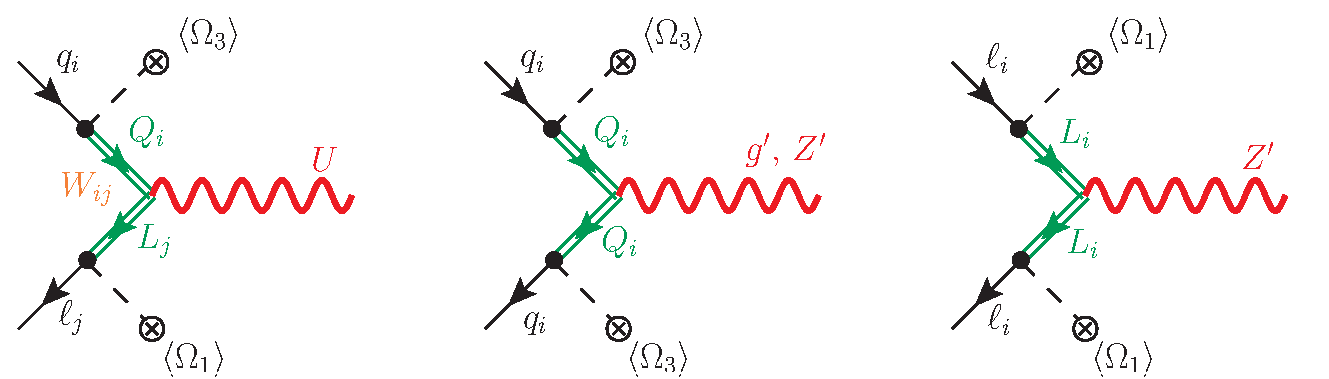
\includegraphics[width=.98\textwidth]{Images/mixing.pdf}
  \captionof{figure}{Diagrammatic representation of the interactions between the SM fermions and the heavy vector-like fermions $\Psi$, induced by the Yukawa couplings to $\Omega_1$ and $\Omega_3$ after symmetry breaking.}
  \label{fig:mixing}
\end{center}

\begin{center}
  \begin{tabular}{|c|c|c|c|c|}
    \hline
    Field & $SU(4)$ & $SU(3)'$ & $SU(2)_L$ & $U(1)'$ \\
    \hline
    \hline
    $q'^i_L$ & $\mathbf{1}$ & $\mathbf{3}$ & $\mathbf{2}$ & $1/6$ \\
    $u'^i_R$ & $\mathbf{1}$ & $\mathbf{3}$ & $\mathbf{1}$ & $2/3$ \\
    $d'^i_R$ & $\mathbf{1}$ & $\mathbf{3}$ & $\mathbf{1}$ & $-1/3$ \\
    $\ell'^i_L$ & $\mathbf{1}$ & $\mathbf{1}$ & $\mathbf{2}$ & $-1/2$ \\
    $e'^i_R$ & $\mathbf{1}$ & $\mathbf{1}$ & $\mathbf{1}$ & $-1$ \\
    \hline
    $\Psi^i_L$ & $\mathbf{4}$ & $\mathbf{1}$ & $\mathbf{2}$ & 0 \\
    $\Psi^i_R$ & $\mathbf{4}$ & $\mathbf{1}$ & $\mathbf{2}$ & 0 \\
    \hline
    \hline
    $H$ & $\mathbf{1}$ & $\mathbf{1}$ & $\mathbf{2}$ & 1/2 \\
    $\Omega_1$ & $\mathbf{\bar 4}$ & $\mathbf{1}$ & $\mathbf{1}$ & $-1/2$ \\
    $\Omega_3$ & $\mathbf{\bar 4}$ & $\mathbf{3}$ & $\mathbf{1}$ & $1/6$ \\
    $\Omega_{15}$ & $\mathbf{15}$ & $\mathbf{1}$ & $\mathbf{1}$ & 0 \\
    \hline
  \end{tabular}
  \captionof{table}{Field content of the 4321 model. The index $i=1,2,3$ runs over generations.}
  \label{tab:fieldcontent}
\end{center}
The mixing between the elementary fermions and the vector-like fermions is described by the Yukawa Lagrangian $\mathcal{L}_Y = \mathcal{L}_{\rm SM-like} + \mathcal{L}_{\rm mix}$, where
\begin{align}
\label{LYUK1}
\mathcal{L}_{\rm SM-like} &=  - \bar{q}'_L \,Y_d \, H d'_R - \bar{q}'_L \,Y_u \, \tilde H u'_R - \bar{\ell}'_L \, Y_e \, H e'_R + \text{h.c.} \, ,  \\
\label{LYUK2}
\mathcal{L}_{\rm mix} &= - \bar {q}'_L \, \lambda_q \, \Omega_3^T \Psi_R - \bar {\ell}'_L \, \lambda_\ell \, \Omega_1^T \Psi_R 
- \bar \Psi_L \left( M + \lambda_{15}\, \Omega_{15} \right) \Psi_R + \text{h.c.} \, .
\end{align}
Here, $\tilde H = i \sigma_2 H^*$, and $Y_{u,d,e}$, $\lambda_{q,\ell,15}$, $M$ are $3 \times 3$ matrices in flavour space.


The vector-like fermions transform under $\mathcal{G}_{\rm 4321}$ as
\begin{equation}
  \Psi_{L,R} = \begin{pmatrix}
    Q'_{L,R} \\
    L'_{L,R}
  \end{pmatrix} \sim (\mathbf{4},\mathbf{1},\mathbf{2},0).
\end{equation}
Under the breaking $SU(4)\to SU(3)_{[4]}\times U(1)_{B-L}$, they decompose as $Q'_{L,R} \sim (\mathbf{3}, \mathbf{2},1/6)$ and $L'_{L,R}\sim(\mathbf{1}, \mathbf{2},-1/2)$. Their vector-like masses are generated by the $M$ term and are split by the VEV of $\Omega_{15}$:
\begin{equation}
  M_Q = M + \frac{\lambda_{15}\, v_{15}}{2\sqrt{6}}\,,  \qquad M_L = M - \frac{3\,\lambda_{15}\,v_{15}}{2\sqrt{6}}\,.
\end{equation}



To comply with flavour constraints, the authors on \cite{DiLuzio2018} employ the following Yukawa textures as a starting point
\begin{align}\label{lamqfs}
\begin{aligned}
\lambda_q &= \hat{\lambda}_q \equiv \text{diag} \left( \lambda^q_{12}, \lambda^q_{12}, \lambda^q_{3} \right)
\, , \\
\lambda_{\ell} &= \hat{\lambda}_{\ell}\,  W^\dagger \equiv
\text{diag} \left( \lambda^{\ell}_{1}, \lambda^{\ell}_{2}, \lambda^{\ell}_{3} \right)
\left(
\begin{array}{ccc}
1 & 0 & 0 \\
0 & \cos \theta_{LQ} & -\sin \theta_{LQ} \\
0 & \sin \theta_{LQ} & \cos \theta_{LQ}
\end{array}
\right) \, , \\ 
\lambda_{15} & \propto \hat{M} \propto \mathbb{1} \, .
\end{aligned}
\end{align}

After the $SU(3)_{[4]}\times SU(3)'\to SU(3)_c$ symmetry breaking, the $6\times6$ fermion mass matrices for the quarks read:
\begin{equation}
  \mathcal{M}_u=
\begin{pmatrix}
V^\dagger\, \hat Y_u\,\frac{v}{\sqrt{2}} &\hat\lambda_q\,\frac{v_3}{\sqrt{2}}\\[2pt]
0 & \hat M_Q
\end{pmatrix}\,,\quad
\mathcal{M}_d=
\begin{pmatrix}
\hat Y_d\,\frac{v}{\sqrt{2}} &\hat\lambda_q\,\frac{v_3}{\sqrt{2}}\\[2pt]
0 & \hat M_Q
\end{pmatrix}\,.
\end{equation}
Similarly, after the $U(1)_{B-L}\times U(1)_{T_R^3}\to U(1)_Y$ symmetry breaking, the $6\times6$ fermion mass matrices for the leptons read:
\begin{align}\label{eq:mass_matrices}
\mathcal{M}_N&=
\begin{pmatrix}
0 &\hat\lambda_\ell\,\frac{v_1}{\sqrt{2}}\\[2pt]
0 & \hat M_L
\end{pmatrix}\,, &
\mathcal{M}_e&=
\begin{pmatrix}
\hat Y_e\,\frac{v}{\sqrt{2}} &\hat\lambda_\ell\,W^\dagger\,\frac{v_1}{\sqrt{2}}\\[2pt]
0 & \hat M_L
\end{pmatrix}\,.
\end{align}
Here, $\hat Y_{u,d,e}$ and $\hat \lambda_{q,\ell}$ are diagonal matrices, $V$ and $W$ are unitary Cabibbo-like mixing matrices, and $M_Q$, $M_L$ are proportional to the identity matrix.

The structure of the mass matrices in Eqs.~\eqref{eq:mass_matrices} allows them to be diagonalized by unitary transformations of the form $\psi_x^\prime = U_x \psi_x$, where $\psi_x$ ($x = q, u, d, \ell, e, N$) denotes a 6-dimensional vector containing both the chiral and vector-like fermions, and the unprimed fields represent the mass eigenstates.\marginpar{For the neutrinos, since we do not include a $\nu_R$ field, the vector $\psi_{N}$ is actually 3-dimensional, containing only the right-handed components $N_R \subset \Psi_R$. For notational simplicity, however, we treat it as a 6-dimensional vector.} 

The chosen flavour structure in Eq.~\eqref{lamqfs} ensures that in the limit $W \to \mathbb{1}$, the mixing is family-specific: each vector-like fermion generation mixes predominantly with only one generation of chiral fermions (up to CKM rotations). At leading order, the unitary mixing matrices are given by:
{\footnotesize
\begin{align*}
  \begin{aligned}
    U_q &\approx \mathcal{R}_{14}(\theta_{q_1}) \, \mathcal{R}_{25}(\theta_{q_2}) \, \mathcal{R}_{36}(\theta_{q_3})\,, &
    U_\ell &\approx \mathcal{R}_{14}(\theta_{\ell_1}) \, \mathcal{R}_{25}(\theta_{\ell_2}) \, \mathcal{R}_{36}(\theta_{\ell_3})\,,\\
    U_u &\approx \mathcal{R}_{14}(\theta_{u_R}) \, \mathcal{R}_{25}(\theta_{c_R}) \, \mathcal{R}_{36}(\theta_{t_R})\,, &
    U_e &\approx
    \begin{pmatrix}
      \mathbb{1} & 0 \\
      0 & W
    \end{pmatrix}
    \mathcal{R}_{14}(\theta_{e_R}) \, \mathcal{R}_{25}(\theta_{\mu_R}) \, \mathcal{R}_{36}(\theta_{\tau_R})\,,\\
    U_d &\approx \mathcal{R}_{14}(\theta_{d_R}) \, \mathcal{R}_{25}(\theta_{s_R}) \, \mathcal{R}_{36}(\theta_{b_R})\,, &
    U_N &\approx
    \begin{pmatrix}
      0 & 0 \\
      0 & W
    \end{pmatrix}.
  \end{aligned}
\end{align*}
}%
Here, we have adopted a flavour basis for the SM $SU(2)_L$ fermion multiplets defined by:
\begin{align}
\label{SU2Lfb}
q^i &=
\begin{pmatrix}
V^*_{ji} \, u_L^j \\
d_L^i
\end{pmatrix},
&&&
\ell^\alpha &=
\begin{pmatrix}
\nu_L^\alpha \\
e_L^\alpha
\end{pmatrix},
\end{align}
where $V$ is the CKM matrix. The mixing angles are related to the Lagrangian parameters by:
\begin{align}\label{eq:mixingangles}
\begin{aligned}
\sin\theta_{q_i} &= \frac{\lambda_i^q v_3}{\sqrt{|\lambda_i^q|^2 v_3^2 + 2 \hat M_Q^2}}\,, &
\cos\theta_{q_i} &= \frac{\sqrt{2} \, \hat M_Q}{\sqrt{|\lambda_i^q|^2 v_3^2 + 2 \hat M_Q^2}}\,, \\[5pt]
\sin\theta_{\ell_i} &= \frac{\lambda_i^\ell v_1}{\sqrt{|\lambda_i^\ell|^2 v_1^2 + 2 \hat M_L^2}}\,, &
\cos\theta_{\ell_i} &= \frac{\sqrt{2} \, \hat M_L}{\sqrt{|\lambda_i^\ell|^2 v_1^2 + 2 \hat M_L^2}}\,, \\[5pt]
\sin\theta_{u_R^i} &= \frac{m_{u_i}}{M_{Q_i}} \tan\theta_{q_i}\,, &
\sin\theta_{d_R^i} &= \frac{m_{d_i}}{M_{Q_i}} \tan\theta_{q_i}\,, \\[5pt]
\sin\theta_{e_R^i} &= \frac{m_{e_i}}{M_{L_i}} \tan\theta_{\ell_i}\,, &
\cos\theta_{f_R^i} &= 1 \quad (f = u, d, e)\,.
\end{aligned}
\end{align}
In these expressions, $m_i$ and $M_i$ denote the physical fermion masses. Up to corrections of $\mathcal{O}(m_i^2 / M_i^2)$, these are given by:
\begin{align}\label{eq:ferm_masses}
\begin{aligned}
M_{L_i} &= \sqrt{\frac{|\lambda_i^\ell|^2 v_1^2}{2} + \hat M_L^2}\,, &
M_{Q_i} &= \sqrt{\frac{|\lambda_i^q|^2 v_3^2}{2} + \hat M_Q^2}\,, \\[2pt]
m_{f_i} &\approx |\hat Y_f^i| \cos\theta_{f_i} \frac{v}{\sqrt{2}} & (f &= u, d, e)\,.
\end{aligned}
\end{align}

The interaction terms of the massive gauge bosons with the fermions in the interaction basis, are readily obtained from the action of the covariant derivative on the fermion fields: 
\begin{align}
\mathcal{L}_L &= \frac{g_4}{\sqrt{2}} \bar{Q}'_L \gamma^\mu L'_L \, U_\mu + \textrm{h.c.}~\nonumber \\
& + g_s \left( \frac{g_4}{g_3} \, \bar{Q}'_L \gamma^\mu T^a Q'_L - \frac{g_3}{g_4} \,\bar{q}'_L \gamma^\mu T^a q'_L \right) g'^a_\mu ~\nonumber \\
&+g_Y \left( \sqrt{\frac{3}{2}}\,\frac{g_4}{g_1}\,Y(Q'_L) \, \bar{Q}'_L \gamma^\mu Q'_L - \sqrt{\frac{2}{3}}\,\frac{g_1}{g_4}\,Y(q'_L) \, \bar{q}'_L \gamma^\mu q'_L \right) Z'_\mu ~\nonumber\\
&+ g_Y \left( \sqrt{\frac{3}{2}}\,\frac{g_4}{g_1}\,Y(L'_L) \, \bar{L}'_L \gamma^\mu L'_L - \sqrt{\frac{2}{3}}\,\frac{g_1}{g_4}\,Y(\ell'_L) \, \bar{\ell}'_L \gamma^\mu \ell'_L \right) Z'_\mu~,\label{eq:coupL}\\[10pt]
\mathcal{L}_R &= \frac{g_4}{\sqrt{2}} \bar{Q}'_R \gamma^\mu L'_R \, U_\mu + \textrm{h.c.}~\nonumber \\
& + g_s \left( \frac{g_4}{g_3} \, \bar{Q}'_R \gamma^\mu T^a Q'_R - \frac{g_3}{g_4}  \,\bar{u}'_R \gamma^\mu T^a u'_R -\frac{g_3}{g_4} \,\bar{d}'_R \gamma^\mu T^a d'_R  \right) g'^a_\mu ~\nonumber \\
&+ g_Y \left( \sqrt{\frac{3}{2}}\,\frac{g_4}{g_1}\,Y(Q'_R) \,\bar{Q}'_R \gamma^\mu Q'_R - \sqrt{\frac{2}{3}}\,\frac{g_1}{g_4}\, Y(u'_R) \, \bar{u}'_R \gamma^\mu u'_R -\sqrt{\frac{2}{3}}\,\frac{g_1}{g_4}\, Y(d'_R) \, \bar{d}'_R \gamma^\mu d'_R \right) Z'_\mu ~\nonumber\\
&+g_Y \left( \sqrt{\frac{3}{2}}\,\frac{g_4}{g_1}\,Y(L'_R) \, \bar{L}'_R \gamma^\mu L'_R - \sqrt{\frac{2}{3}}\,\frac{g_1}{g_4}\,
Y(e'_R) \, \bar{e}'_R \gamma^\mu e'_R \right) Z'_\mu~,\label{eq:coupR}
\end{align}
where we left implicit the SM hypercharges: 
$Y(Q'_{L}) = Y(Q'_{R}) = Y(q'_{L}) = \tfrac{1}{6}$, $Y(u'_R) = \tfrac{2}{3}$, $Y(d'_R) = -\tfrac{1}{3}$, 
$Y(L'_L) = Y(L'_R) = Y(\ell'_L) = -\tfrac{1}{2}$ and $Y(e'_R) = -1$.   

To express the interactions above in the fermion mass basis, we collect the fields in 6-dimensional multiplets, $\psi_x$ ($x=q,u,d,\ell,e$), and apply the unitary transformations defined in equation~\ref{eq:RotMass}. Neglecting right-handed rotations, suppressed by the small masses of the SM fermions, we have
\begin{align}
\begin{aligned}
\mathcal{L}_U&=\frac{g_4}{\sqrt{2}}\,U_\mu\left[\beta\,\bar \psi_q\gamma^\mu \psi_\ell+W\,\bar Q_R\gamma^\mu L_R\right]+h.c.\,,\\
\mathcal{L}_{g^\prime}&= g_s\,\frac{g_4}{g_3}\,g^{\prime\,a}_\mu\left[\kappa_q\,\bar \psi_q\gamma^\mu\,T^a\, \psi_q+\kappa_u\,\bar \psi_u\gamma^\mu\,T^a\, \psi_u+\kappa_d\,\bar \psi_d\gamma^\mu\,T^a\, \psi_d\right]\,,\\
\mathcal{L}_{Z^\prime}&=\frac{g_Y}{2\sqrt{6}}\,\frac{g_4}{g_1}\,Z_\mu^\prime\left[\zeta_q\,\bar \psi_q\gamma^\mu \psi_q+\zeta_u\,\bar \psi_u\gamma^\mu \psi_u
\right.
\\&\qquad
\left.
+\zeta_d\,\bar \psi_d\gamma^\mu \psi_d-3\,\zeta_\ell\,\bar \psi_\ell\gamma^\mu \psi_\ell-3\,\zeta_e\,\bar \psi_e\gamma^\mu \psi_e\right]\,,\label{eq:LLmbS}
\end{aligned}
\end{align}
with ($A,B=4,5,6$ and $\alpha,\beta=1,\dots,6$)
\begin{align}
\begin{aligned}
\beta^{\alpha\beta}&= \big[U_q\big]^*_{A\alpha}\big[W\big]_{AB} \big[U_\ell\big]_{B\beta}\,,\\
\kappa_q^{\alpha\beta}&= \big[U_q\big]^*_{A\alpha} \big[U_q\big]_{A\beta}-\frac{g_3^2}{g_4^2}\,\delta_{\alpha\beta}\,,&\kappa_u\approx\kappa_d&\approx
\begin{pmatrix}
0 & 0\\
0 & \mathbb{1}_{3\times3}
\end{pmatrix}
-\frac{g_3^2}{g_4^2}\,\mathbb{1}_{6\times6}\,,\\
\zeta_q^{\alpha\beta}&= \big[U_q\big]^*_{A\alpha} \big[U_q\big]_{A\beta}-\frac{2\,g_1^2}{3\,g_4^2}\,\delta_{\alpha\beta}\,,& \zeta_u\approx\zeta_d&\approx
\begin{pmatrix}
0 & 0\\
0 & \mathbb{1}_{3\times3}
\end{pmatrix}
-\frac{2\,g_1^2}{3\,g_4^2}\,\mathbb{1}_{6\times6}\,,\\
\zeta_\ell^{\alpha\beta}&= \big[U_\ell\big]^*_{A\alpha} \big[U_\ell\big]_{A\beta}-\frac{2\,g_1^2}{3\,g_4^2}\,\delta_{\alpha\beta}\,,& \zeta_e&\approx
\begin{pmatrix}
0 & 0\\
0 & \mathbb{1}_{3\times3}
\end{pmatrix}
-\frac{2\,g_1^2}{3\,g_4^2}\,\mathbb{1}_{6\times6}\,.
\end{aligned}
\end{align}
Note in particular that the $W$ matrix cancels by unitarity in the $Z^\prime$ and $g^\prime$ interactions. This is a key result of the assumed flavour structure. Assuming $W=\mathcal{R}_{56}(\theta_{LQ})$ and no CP violation in the mixing angles, the left-handed couplings can be rewritten as
\begin{align}\label{eq:Beta}
\beta &\approx
\begin{pmatrix}
  \diag( s_{q_1}s_{\ell_1}, s_{q_2}s_{\ell_2}, s_{q_3}s_{\ell_3} ) W& -\diag( s_{q_1}c_{\ell_1}, s_{q_2}c_{\ell_2}, s_{q_3}c_{\ell_3} ) W \\
  \diag( c_{q_1}s_{\ell_1}, c_{q_2}s_{\ell_2}, c_{q_3}s_{\ell_3} ) W & -\diag( c_{q_1}c_{\ell_1}, c_{q_2}c_{\ell_2}, c_{q_3}c_{\ell_3} ) W
\end{pmatrix},
\\
\kappa_q &\approx
\begin{pmatrix}
  \diag( s_{q_1}^2, s_{q_2}^2, s_{q_3}^2 ) & -\frac{1}{2}\diag( s_{2q_1}, s_{2q_2}, s_{2q_3} ) \\
  -\frac{1}{2}\diag( s_{2q_1}, s_{2q_2}, s_{2q_3} )  & \diag( c_{q_1}^2, c_{q_2}^2, c_{q_3}^2 )
\end{pmatrix}
-\frac{g_3^2}{g_4^2}\,\mathbb{1}_{6\times6},
\\
\zeta_q &\approx
\begin{pmatrix}
  \diag( s_{q_1}^2, s_{q_2}^2, s_{q_3}^2 ) & -\frac{1}{2}\diag( s_{2q_1}, s_{2q_2}, s_{2q_3} ) \\
  -\frac{1}{2}\diag( s_{2q_1}, s_{2q_2}, s_{2q_3} )  & \diag( c_{q_1}^2, c_{q_2}^2, c_{q_3}^2 )
\end{pmatrix}
-\frac{2\,g_1^2}{3\,g_4^2}\,\mathbb{1}_{6\times6},
\\
\zeta_\ell &\approx
\begin{pmatrix}
  \diag( s_{\ell_1}^2, s_{\ell_2}^2, s_{\ell_3}^2 ) & -\frac{1}{2}\diag( s_{2\ell_1}, s_{2\ell_2}, s_{2\ell_3} ) \\
  -\frac{1}{2}\diag( s_{2\ell_1}, s_{2\ell_2}, s_{2\ell_3} )  & \diag( c_{\ell_1}^2, c_{\ell_2}^2, c_{\ell_3}^2 )
\end{pmatrix}
-\frac{2\,g_1^2}{3\,g_4^2}\,\mathbb{1}_{6\times6}.
\label{eq:LLmbE}
\end{align}

